\documentclass[a4paper, czech]{article}

\title{
    \begin{framed}
        \setstretch{1.5}
        {\large Audio elektronika (BPC/BKC-AUD)}\\
        Laboratorní úloha č. 4 (protokol)\\
        \textbf{Aktivní výhybka pro dva satelity a subwoofer}
    \end{framed}
    }
\author{Karolína A. Šebestová}
\date{10. 4. 2026, 11:00}

\usepackage[czech]{babel}
\usepackage{indentfirst}
\usepackage{graphicx}
\usepackage{float}
\usepackage[margin=1.5cm]{geometry}
\usepackage{booktabs}
\usepackage{amsmath}
\usepackage{multirow}
\usepackage{colortbl}
\usepackage{framed} % \begin{framed}
\usepackage{setspace} % \setstretch{}
\usepackage{siunitx}
\usepackage{multirow}
\usepackage{xcolor}

\sisetup{locale = DE}

\begin{document}

\maketitle

\section{Měření}

\subsection{Měření modulové kmitočtové charakteristiky lineárního nefiltrovaného výstupu.}

\begin{equation}
    A_\text{U} = \textcolor{teal}{20 \cdot \log \frac{U_2}{U_1}} = 20 \cdot \log \frac{370}{500} = \underline{\underline{-2{,}62\,\text{dB}}}
\end{equation}

\begin{table}[H]
    \catcode`\-=12
    \centering
    \caption{Modulová kmitočtová charakteristika lineárního výstupu}
    \begin{tabular}{ccc}
        \toprule
        $f$ \textbf{[Hz]} & $U_2$ \textbf{[mV]} & $A_u$ \textbf{[dB]} \\
        \midrule
        10     & 370     & -2,62   \\
        15     & 425     & -1,41   \\
        20     & 450     & -0,92   \\
        30     & 473     & -0,48   \\
        50     & 487     & -0,23   \\
        70     & 491     & -0,16   \\
        100    & 493     & -0,12   \\
        200    & 495     & -0,09   \\
        500    & 496     & -0,07   \\
        700    & 496     & -0,07   \\
        1 000  & 496     & -0,07   \\
        2 000  & 496     & -0,07   \\
        5 000  & 496     & -0,07   \\
        7 000  & 496     & -0,07   \\
        10 000 & 496     & -0,07   \\
        20 000 & 496     & -0,07   \\
        30 000 & 497     & -0,05  \\
        \bottomrule
    \end{tabular}
\end{table}

\begin{figure}[H]
    \centering
    
\includegraphics[width=\textwidth]{grafy/graf1.pdf}
    \caption{Modulová kmitočtová charakteristika lineárního výstupu}
\end{figure}

\subsection{Měření modulové kmitočtové charakteristiky horní propusti pro levý satelit}

\begin{table}[H]
    \catcode`\-=12
    \centering
    \caption{Modulová kmitočtová charakteristika horní propusti}
    \begin{tabular}{ccccccc}
        \toprule
        \multirow{2}{*}{\setstretch{2}$f$ \textbf{[Hz]}}& \multicolumn{2}{c}{$f_m$ = 80\,Hz} & \multicolumn{2}{c}{$f_m$ = 120\,Hz} & \multicolumn{2}{c}{$f_m$ = 160\,Hz} \\
        \cmidrule(rl){2-3}
        \cmidrule(rl){4-5}
        \cmidrule(rl){6-7}
         & $U_2$ \textbf{[mV]} & $A_u$ \textbf{[dB]} & $U_2$ \textbf{[mV]} & $A_u$ \textbf{[dB]} & $U_2$ \textbf{[mV]} & $A_u$ \textbf{[dB]} \\
        \midrule
        10     & 0,6            & -58,42        & 3,7            & -42,62         & 0,13           & -71,70         \\
        20     & 5,6            & -39,02        & 17,1           & -29,32         & 0,48           & -60,35         \\
        30     & 19,6           & -28,13        & 36,7           & -22,69         & 1,7            & -49,37         \\
        50     & 88,3           & -15,06        & 83,5           & -15,55         & 8,1            & -35,81         \\
        70     & 215            & -7,33         & 130            & -11,70         & 22,1           & -27,09         \\
        100    & 404            & -1,85         & 194            & -8,22          & 62,5           & -18,06         \\
        150    & 493            & -0,12         & 276            & -5,16          & 189            & -8,45          \\
        200    & 500            & 0,00          & 333            & -3,53          & 343            & -3,27          \\
        250    & 499            & -0,02         & 373            & -2,55          & 440            & -1,11          \\
        300    & 497            & -0,05         & 400            & -1,94          & 479            & -0,37          \\
        400    & 495            & -0,09         & 434            & -1,23          & 497            & -0,05         \\
        \bottomrule
    \end{tabular}
\end{table}

\begin{figure}[H]
    \centering
    
\includegraphics[width=\textwidth]{grafy/graf2.pdf}
    \caption{Modulová kmitočtová charakteristika horní propusti}
\end{figure}

$f_{m80} = 93,7\,\text{Hz}$

$f_{m120} = 178,6\,\text{Hz}$

$f_{m160} = 205,1\,\text{Hz}$

$S_{80} = 63,0\,\text{dB/dek}$

$S_{160} = 60,0\,\text{dB/dek}$

$S_{120}$ nebylo možné určit, protože charakteristika není lineární.

\subsection{Měření průběhu zesílení subwooferu v závislosti na nastavení přepínače zesílení}

\begin{table}[H]
    \catcode`\-=12
    \centering
    \caption{Závislost zesílení subwooferu na nastavení přepínače zesílení}
    \begin{tabular}{ccc}
        \toprule
        nastavené & \multirow{3}{*}{$U_2$ \textbf{[mV]}} & \multirow{3}{*}{$A_u$ \textbf{[dB]}} \\
        zesílení &  &  \\
        \textbf{[dB]} &  &  \\
        \midrule
        $+$9                    & 1 410   & 9,00    \\
        $+$6                    & 1 000   & 6,02    \\
        $+$3                    & 709     & 3,03    \\
        0                       & 504     & 0,07    \\
        $-$3                    & 357     & -2,93   \\
        $-$6                    & 254     & -5,88   \\
        \bottomrule
    \end{tabular}
\end{table}

\begin{figure}[H]
    \centering
    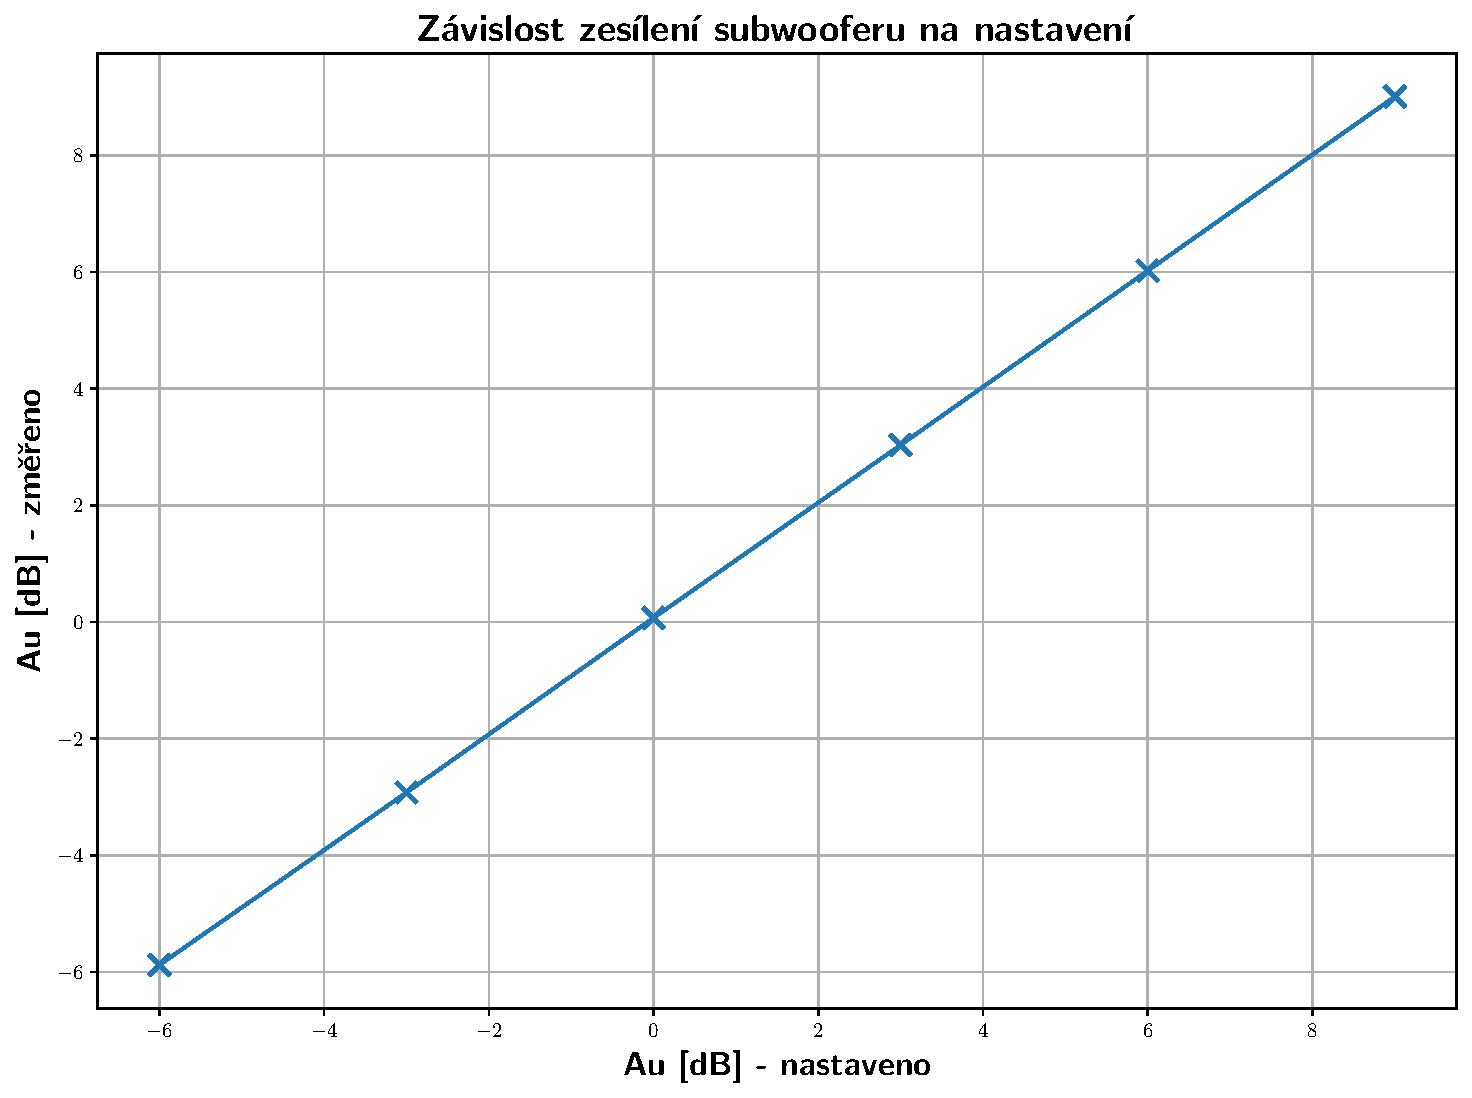
\includegraphics[width=\textwidth]{grafy/graf3.pdf}
    \caption{Závislost zesílení subwooferu na nastavení přepínače zesílení}
\end{figure}

\subsection{Měření modulové kmitočtové charakteristiky výstupu pro subwoofer.}

\begin{table}[H]
    \catcode`\-=12
    \centering
    \caption{Modulová kmitočtová charakteristika dolní propusti}
    \begin{tabular}{ccccccc}
        \toprule
        \multirow{2}{*}{\setstretch{2} $f$ \textbf{[Hz]}} & \multicolumn{2}{c}{$f_m$ = 80\,Hz} & \multicolumn{2}{c}{$f_m$ = 120\,Hz} & \multicolumn{2}{c}{$f_m$ = 160\,Hz} \\
        \cmidrule(rl){2-3}
        \cmidrule(rl){4-5}
        \cmidrule(rl){6-7}
         & $U_2$ \textbf{[mV]} & $A_u$ \textbf{[dB]} & $U_2$ \textbf{[mV]} & $A_u$ \textbf{[dB]} & $U_2$ \textbf{[mV]} & $A_u$ \textbf{[dB]} \\
        \midrule
        10     & 381            & -2,36         & 380            & -2,38          & 375            & -2,50          \\
        20     & 456            & -0,80         & 456            & -0,80          & 452            & -0,88          \\
        30     & 476            & -0,43         & 478            & -0,39          & 477            & -0,41          \\
        50     & 474            & -0,46         & 502            & 0,03           & 494            & -0,10          \\
        70     & 377            & -2,45         & 499            & -0,02          & 503            & 0,05           \\
        100    & 190            & -8,40         & 404            & -1,85          & 499            & -0,02          \\
        150    & 63,2           & -17,97        & 185            & -8,64          & 383            & -2,32          \\
        200    & 27,6           & -25,16        & 86,1           & -15,28         & 222            & -7,05          \\
        250    & 14,3           & -30,87        & 46,1           & -20,71         & 125            & -12,04         \\
        300    & 8,36           & -35,54        & 27,3           & -25,26         & 75,7           & -16,40        \\
        \bottomrule
    \end{tabular}
\end{table}

\begin{figure}[H]
    \centering
    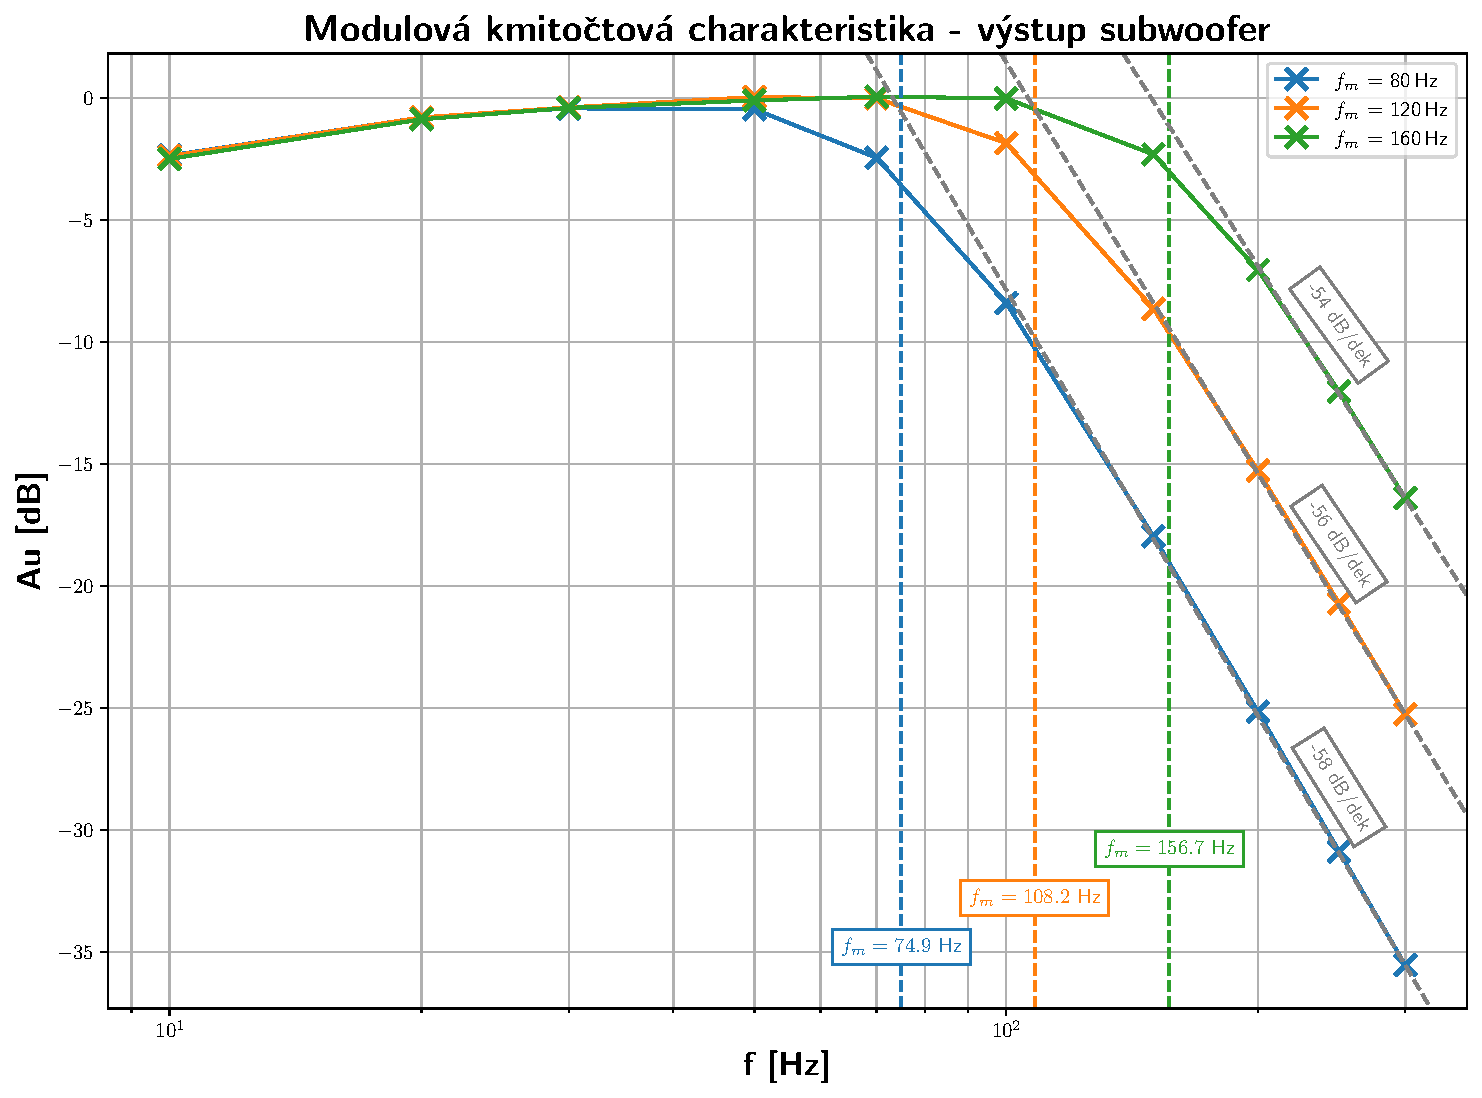
\includegraphics[width=\textwidth]{grafy/graf4.pdf}
    \caption{Modulová kmitočtová charakteristika dolní propusti}
\end{figure}

\section{Použité měřící přístroje}

\begin{itemize}
    \item \textbf{GEN} nízkofrekvenční funkční generátor Agilent 33220A
    \item \textbf{OSC} digitální osciloskop Agilent DSO3102A 100 MHz
    \item \textbf{NZ} napájecí zdroj MCP M10-DP-305E (napájení přípravku $\pm$ 15V)
    \item \textbf{NMV} nízkofrekvenční milivoltmetr Grundig MV100
    \item měřený přípravek „Přesaditelná aktivní výhybka pro subwoofer a satelity“
    \item propojovací vodiče 4 x BNC-BNC
    \item 2 x rozbočovací „T člen“ BNC
\end{itemize}

\section{Závěr}

V prvním bodě měření byla změřena modulová kmitočtová charakteristika lineárního nefiltrovaného výstupu.
Charakteristika se linearizuje přibližně od kmitočtu 100\,Hz.

Ve druhém bodě měření byla proměřena modulová kmitočtová charakteristika horní propusti pro satelit pro všechny tři nastavitelné mezní kmitočty.
Naměřené mezní kmitočty se od nastavených hodnot liší. Pro $f_m = 80$\,Hz byl naměřen mezní kmitočet 93{,}7\,Hz (odchylka $+13{,}7$\,Hz), pro $f_m = 120$\,Hz bylo naměřeno 178{,}6\,Hz (odchylka $+58{,}6$\,Hz) a pro $f_m = 160$\,Hz bylo naměřeno 205{,}1\,Hz (odchylka $+45{,}1$\,Hz).
Největší odchylka nastala pro $f_m = 120$\,Hz, přičemž charakteristika v tomto případě nebyla lineární a strmost nebylo možné určit.
Použité Besselovy filtry třetího řádu by měly dosahovat strmosti 60\,dB/dek (18\,dB/okt); naměřená strmost pro $f_m = 80$\,Hz je 63\,dB/dek, pro $f_m = 160$\,Hz odpovídá teoretické hodnotě 60\,dB/dek.
Odchylky mohou být způsobeny tolerancí součástek nebo nepřesností měřicích přístrojů.

Ve třetím bodě měření byla proměřena závislost zesílení subwooferu na nastavení přepínače zesílení.
Naměřené hodnoty velmi těsně kopírují nastavené hodnoty, maximální odchylka činí pouze 0{,}12\,dB.
Závislost je lineární bez výraznějších odchylek.

Ve čtvrtém bodě měření byla proměřena modulová kmitočtová charakteristika dolní propusti výstupu pro subwoofer pro všechny tři nastavitelné mezní kmitočty.
Naměřené mezní kmitočty se od nastavených hodnot liší méně než v případě horní propusti -- odečtené hodnoty jsou přibližně 75{,}0\,Hz, 108{,}2\,Hz a 156{,}7\,Hz pro nastavené $f_m = 80$, 120 a 160\,Hz.
Odečtené strmosti ($-58$, $-56$ a $-54$\,dB/dek) se od teoretické hodnoty 60\,dB/dek pro Besselův filtr třetího řádu liší o 2 až 6\,dB/dek.
Tyto odchylky mohou být opět způsobeny tolerancí součástek nebo měřicích přístrojů.

\end{document}